
%\begin{frame}{\citetitle{MarcoNuno_ReporteTecnico2022}  \footnotemark{} (1)}
%\begin{frame}{\citetitle{MarcoNuno_ReporteTecnico2022}  \footnote{\fullcite{MarcoNuno_ReporteTecnico2022}} (1)}
\begin{frame}{\citetitle{MarcoNuno_ReporteTecnico2022}$^*$ (1)}
%\begin{frame}{}
%\footfullcite*{MarcoNuno_ReporteTecnico2022}
\begin{columns}
\begin{column}{0.6\textwidth}
	\begin{itemize}  %del cuerpo académico Acuicultura Sustentable (UTMTB-CA-1)
        \item Proyecto desarrollado  en colaboración con investigadores de la Universidad Tecnológica del Mar de Tamaulipas Bicentenario (UTMarT)
		\item Desarrollar una herramienta para automatizar el conteo de microalgas, específicamente de las especies \textit{Isochrysis galbana} e \textit{Chaetoceros muelleri}
        \item Herramientas Software a utilizar: Python (PC), OpenCV, y Android Studio
        \item Herramientas Hardwware a utilizar: Teléfono inteligente (para captura imágenes), adaptador teléfono-microscopio
	\end{itemize}
\end{column}
\begin{column}{0.4\textwidth}  
\begin{center}
     \begin{tabular}{cc}
         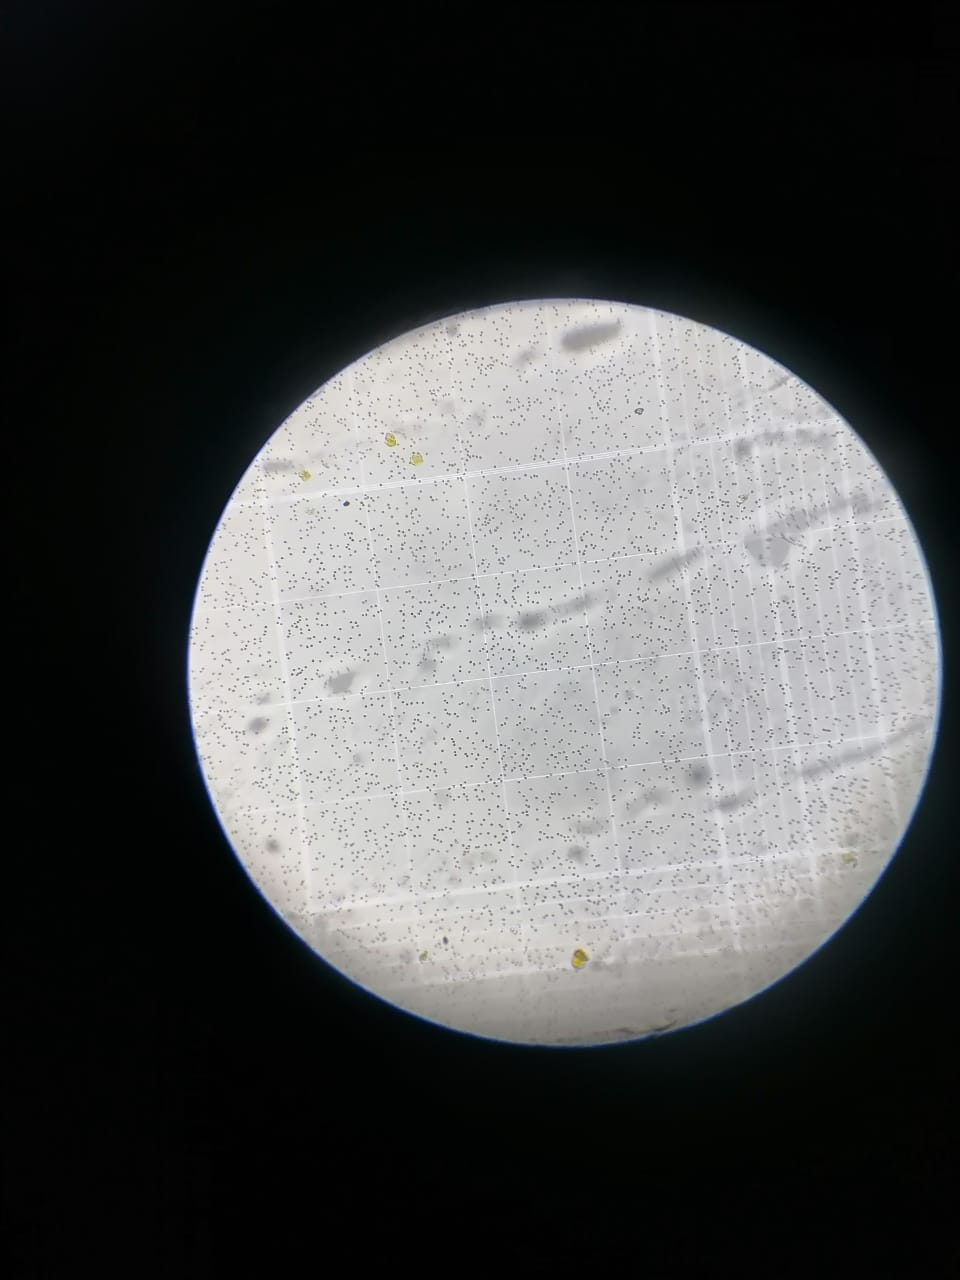
\includegraphics[width=0.68\textwidth]{2022_ConteoMicroAlgas/figs/MicroAlgas01}\\         
      \end{tabular}
\end{center}
\end{column} 
\end{columns} 


%\footnotetext[1]{\fullcite{MarcoNuno_ReporteTecnico2022}}
%\setcounter{footnote}{0}
%\footnotetext{\fullcite{MarcoNuno_ReporteTecnico2022}}
%\footfullcite{MarcoNuno_ReporteTecnico2022}
\footfullcite*{MarcoNuno_ReporteTecnico2022}
\end{frame}


\begin{frame}{\citetitle{MarcoNuno_ReporteTecnico2022} (2)}
\begin{columns}
\begin{column}{0.6\textwidth}
Problemas Encontrados:
\begin{itemize}
        \item Rotación de la rejilla de referencia
        \item Nivel de acercamiento es variable
		\item Imágenes con ruido, distancia de captura variable, regionres con desenfoque 
        \item Problemas de contraste (complica encontrar las lineas)
        \item Cuando hay muchas algas, hay grupos de algas que suelen formar lineas falsas
	\end{itemize}
\end{column}
\begin{column}{0.4\textwidth}  
\begin{center}
     \begin{tabular}{cc}
         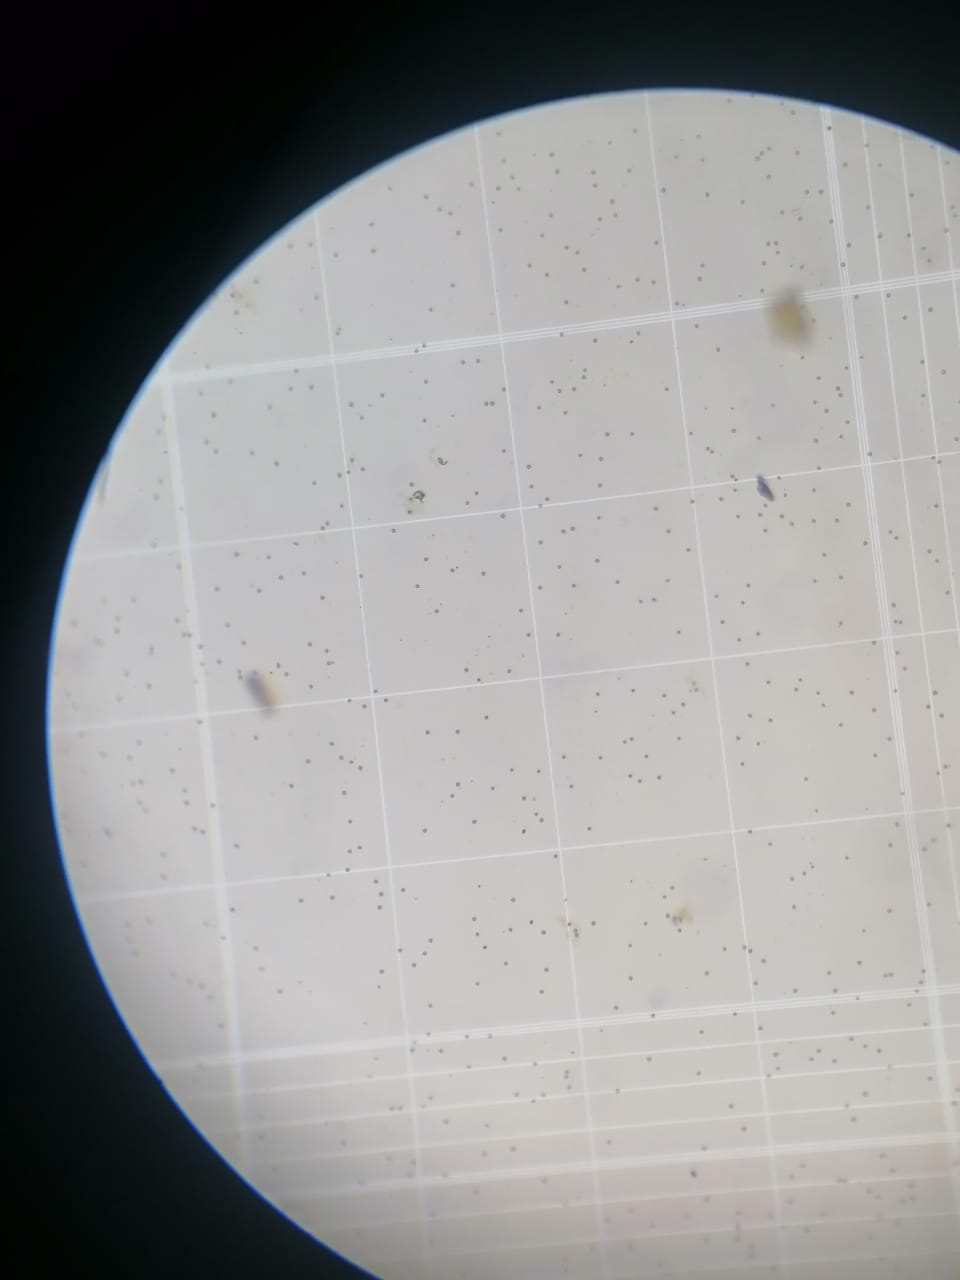
\includegraphics[width=0.38\textwidth]{2022_ConteoMicroAlgas/figs/CuadranteA}&
         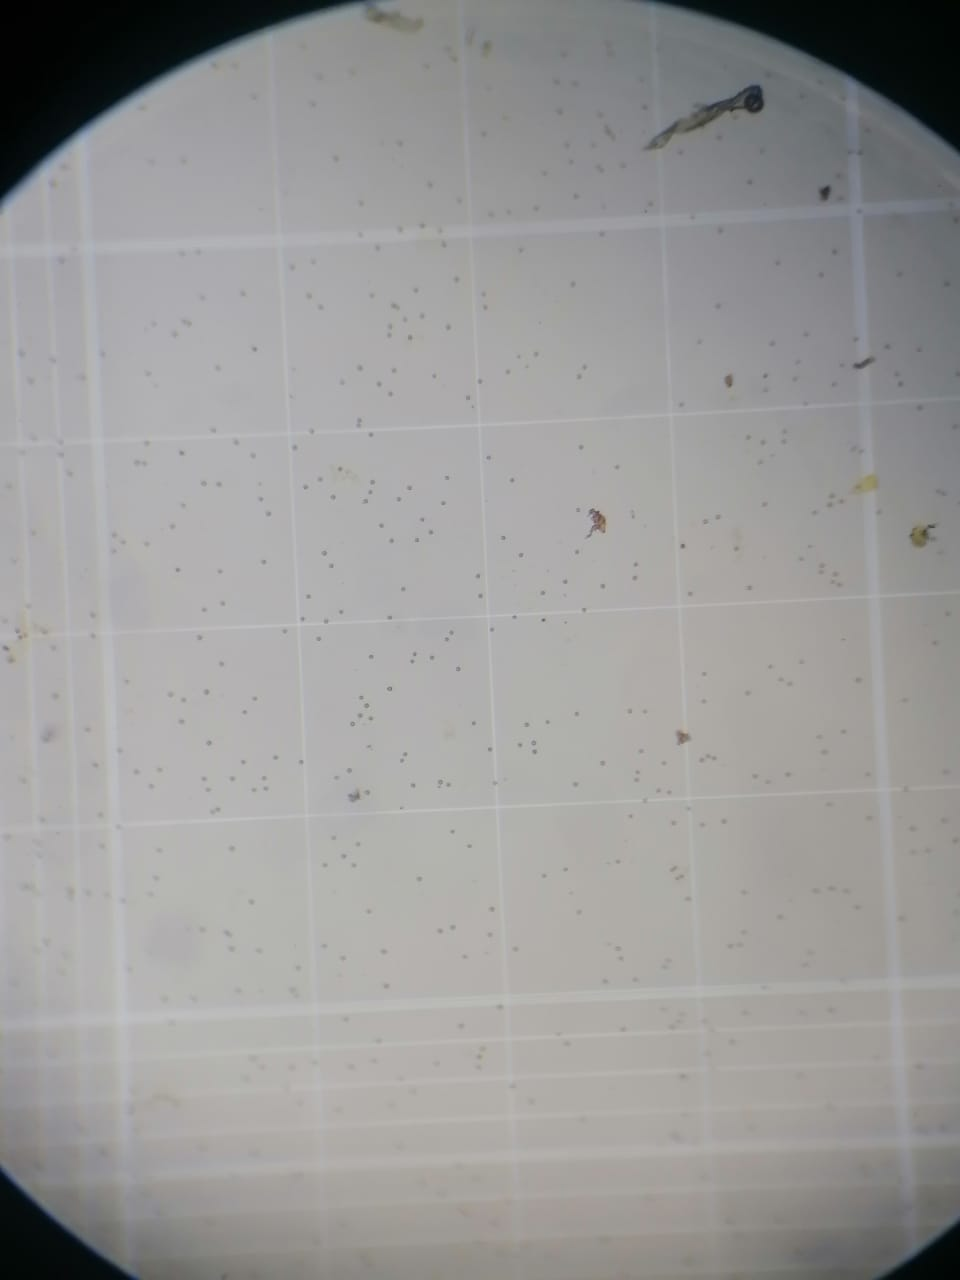
\includegraphics[width=0.38\textwidth]{2022_ConteoMicroAlgas/figs/CuadranteB}\\
         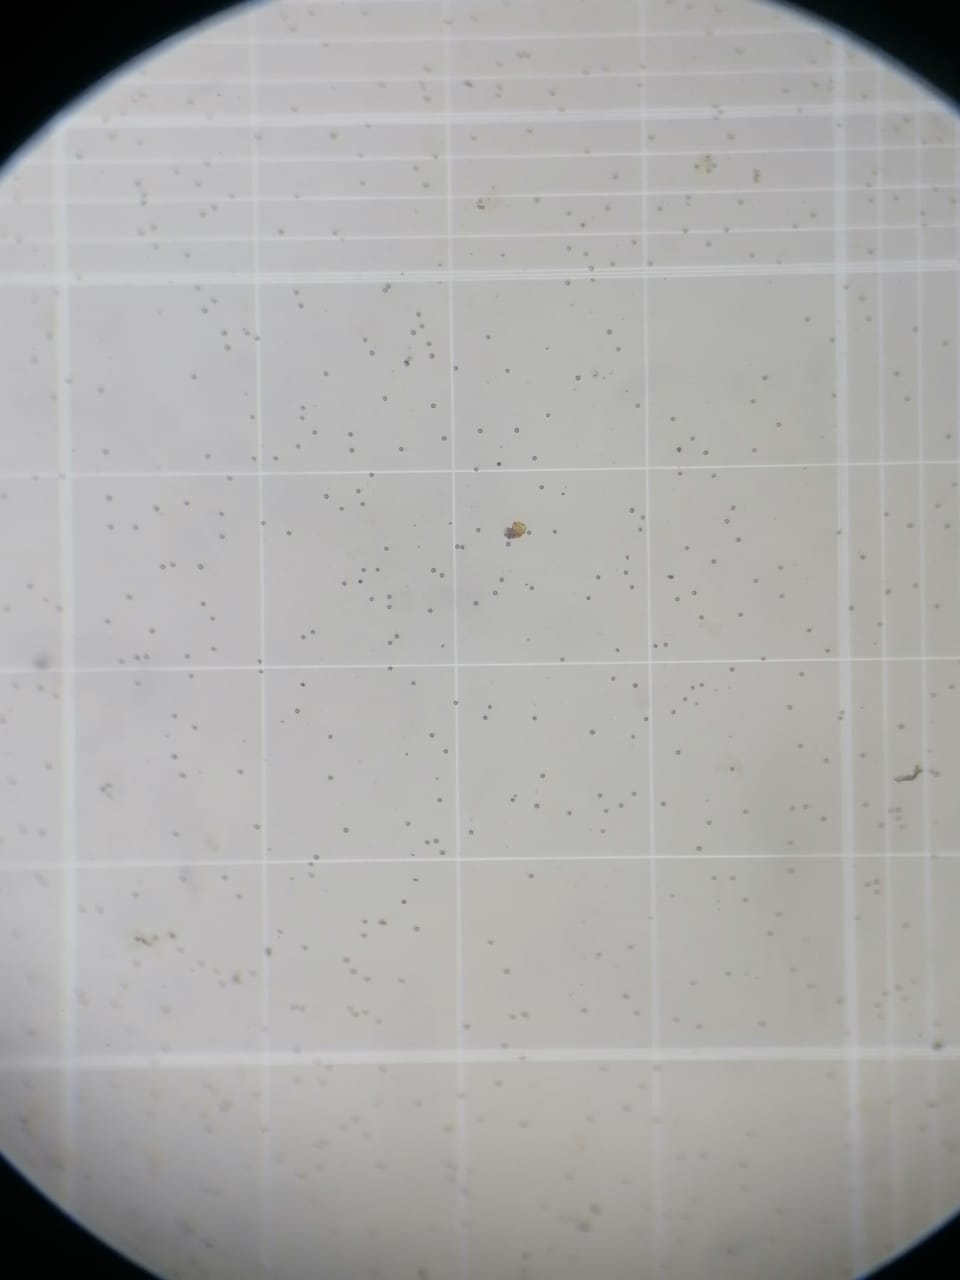
\includegraphics[width=0.38\textwidth]{2022_ConteoMicroAlgas/figs/CuadranteC}&
         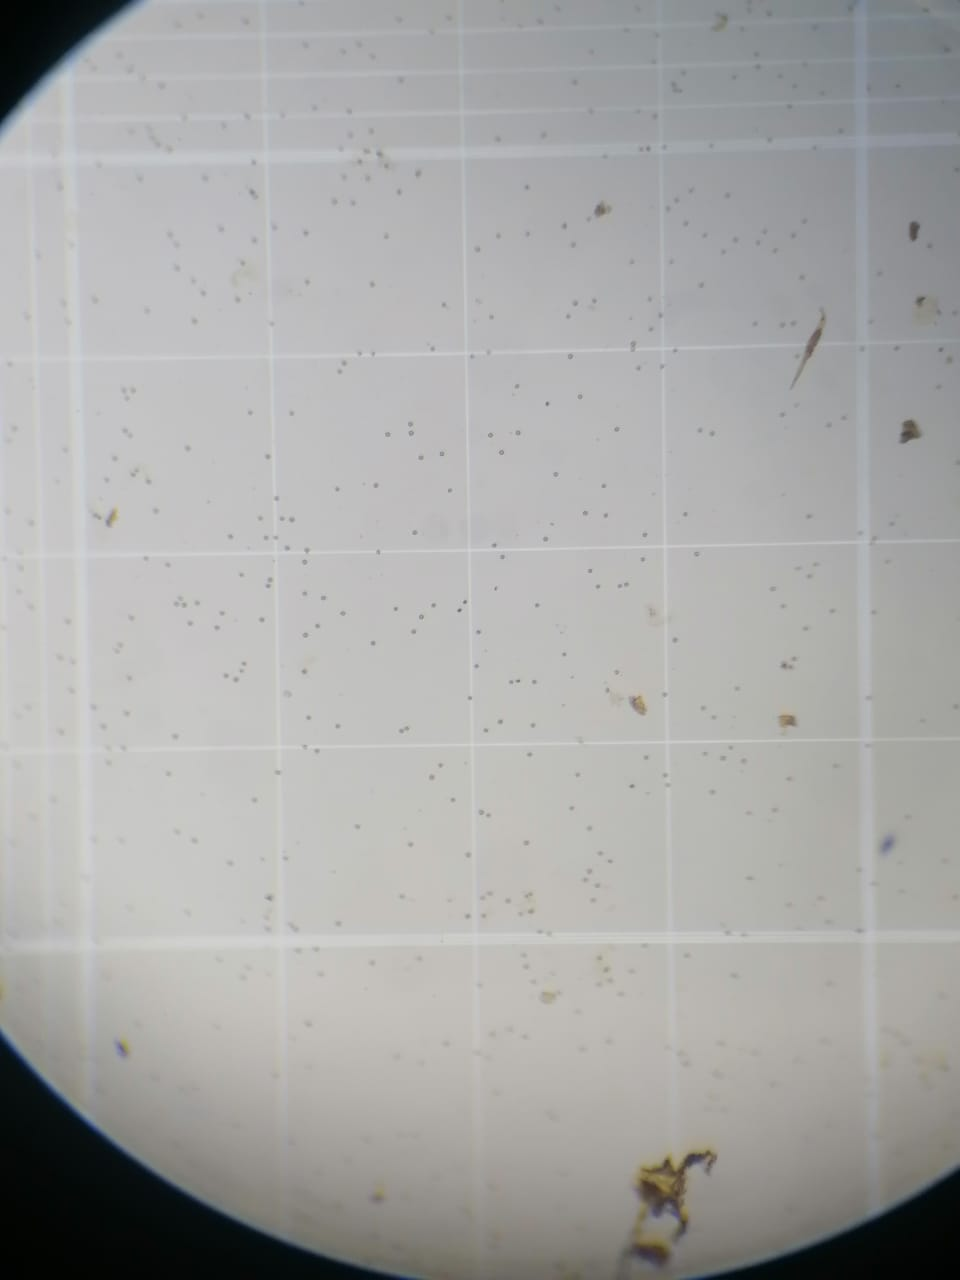
\includegraphics[width=0.38\textwidth]{2022_ConteoMicroAlgas/figs/CuadranteD}\\
          \end{tabular}
\end{center}
\end{column} 
\end{columns} 
\end{frame}


\begin{frame}{\citetitle{MarcoNuno_ReporteTecnico2022} (3)}
\begin{columns}
\begin{column}{0.50\textwidth}
Fases del algoritmo en desarrollo:
\begin{itemize}
		\item Binalizar las imágenes y aplicar un algoritmo de detección de bordes
        \item Encontrar las líneas mediante los algoritmos de Hough Standard y Probabilístico
        \item Analizar las líneas encontradas para determinar aquellas que deben descartarse 
        \item Efectuar un enmascarado de regiones para aislar solo la rejilla delimitadora
        \item Llevar a cabo el conteo de las algas a partir de los contornos de la imágen de bordes
	\end{itemize}
\end{column}
\begin{column}{0.50\textwidth}  
\begin{center}
     \begin{tabular}{ccc}
         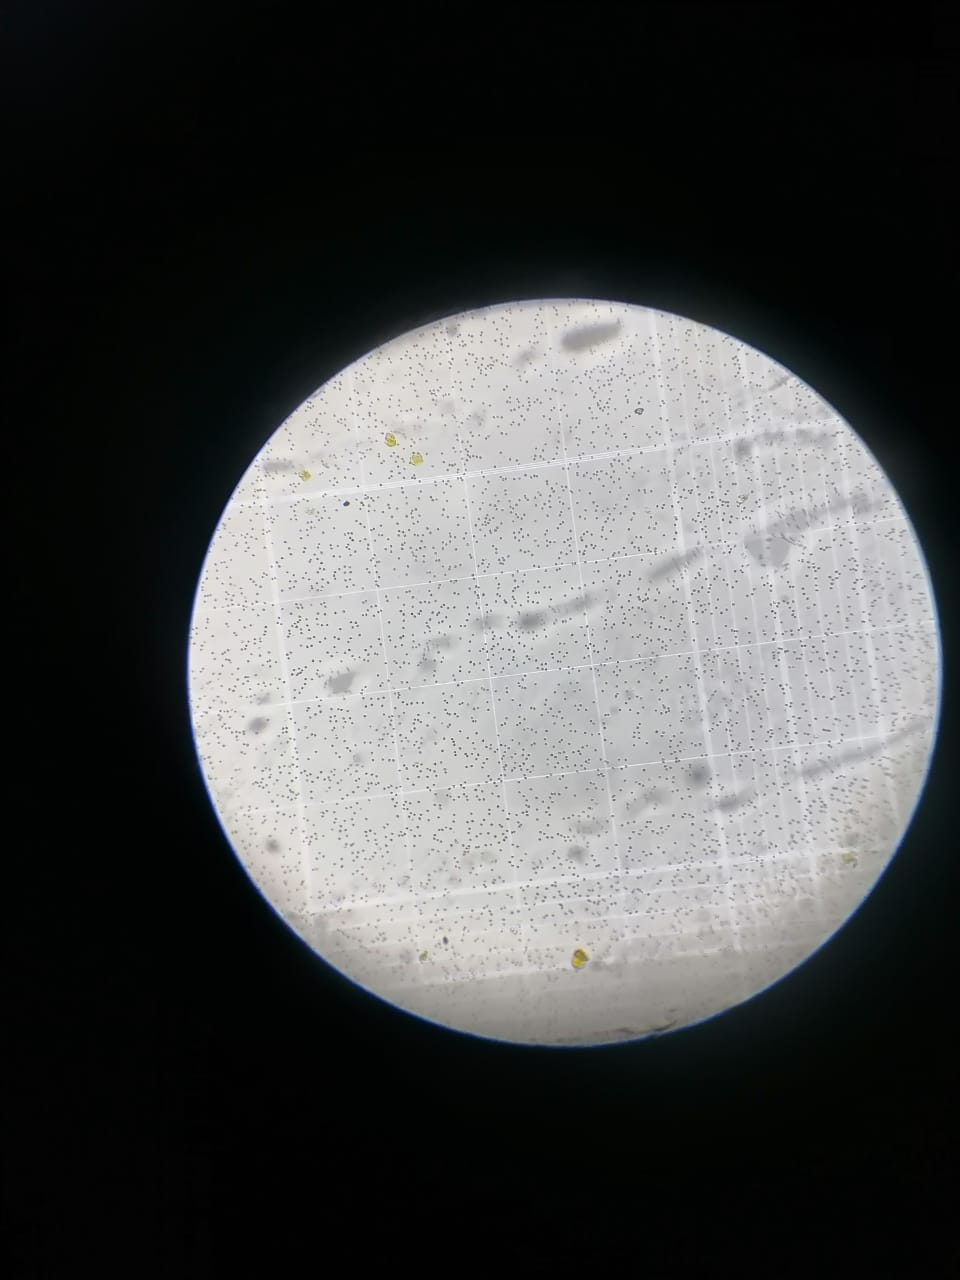
\includegraphics[width=0.31\textwidth]{2022_ConteoMicroAlgas/figs/MicroAlgas01}&
         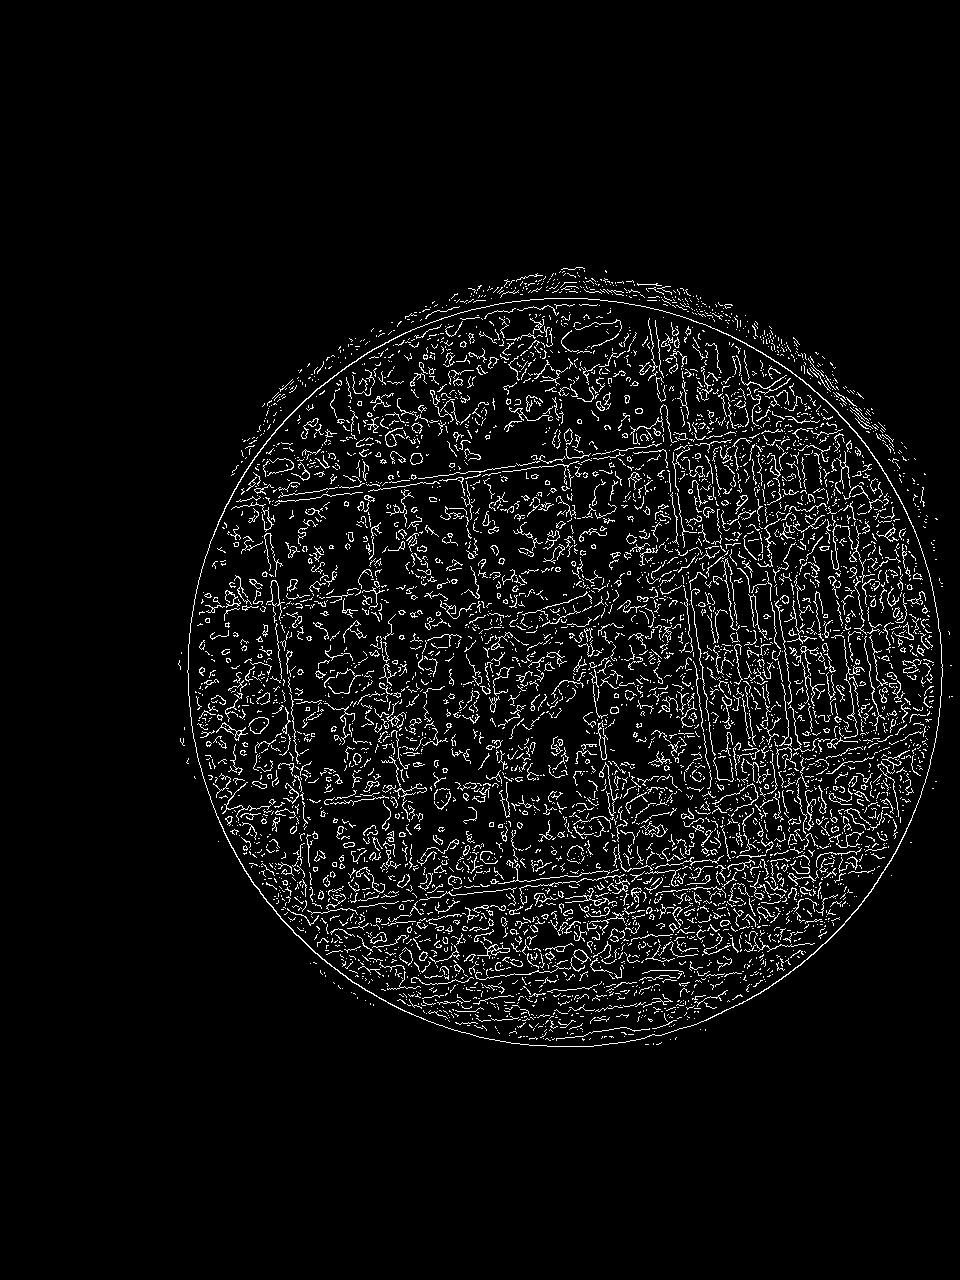
\includegraphics[width=0.31\textwidth]{2022_ConteoMicroAlgas/figs/02_Canny}&
         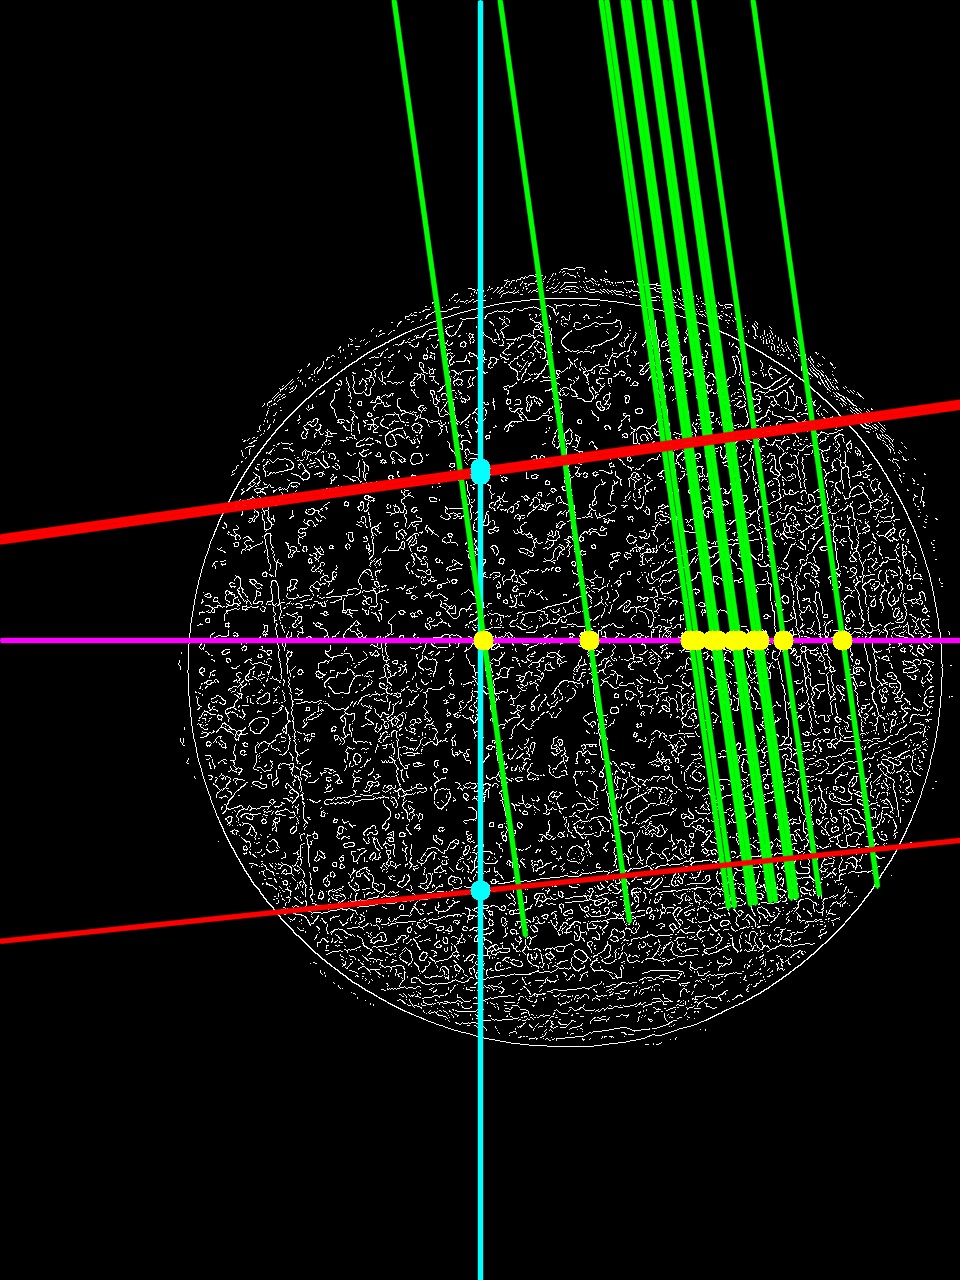
\includegraphics[width=0.31\textwidth]{2022_ConteoMicroAlgas/figs/03_LineasEstandar}\\
         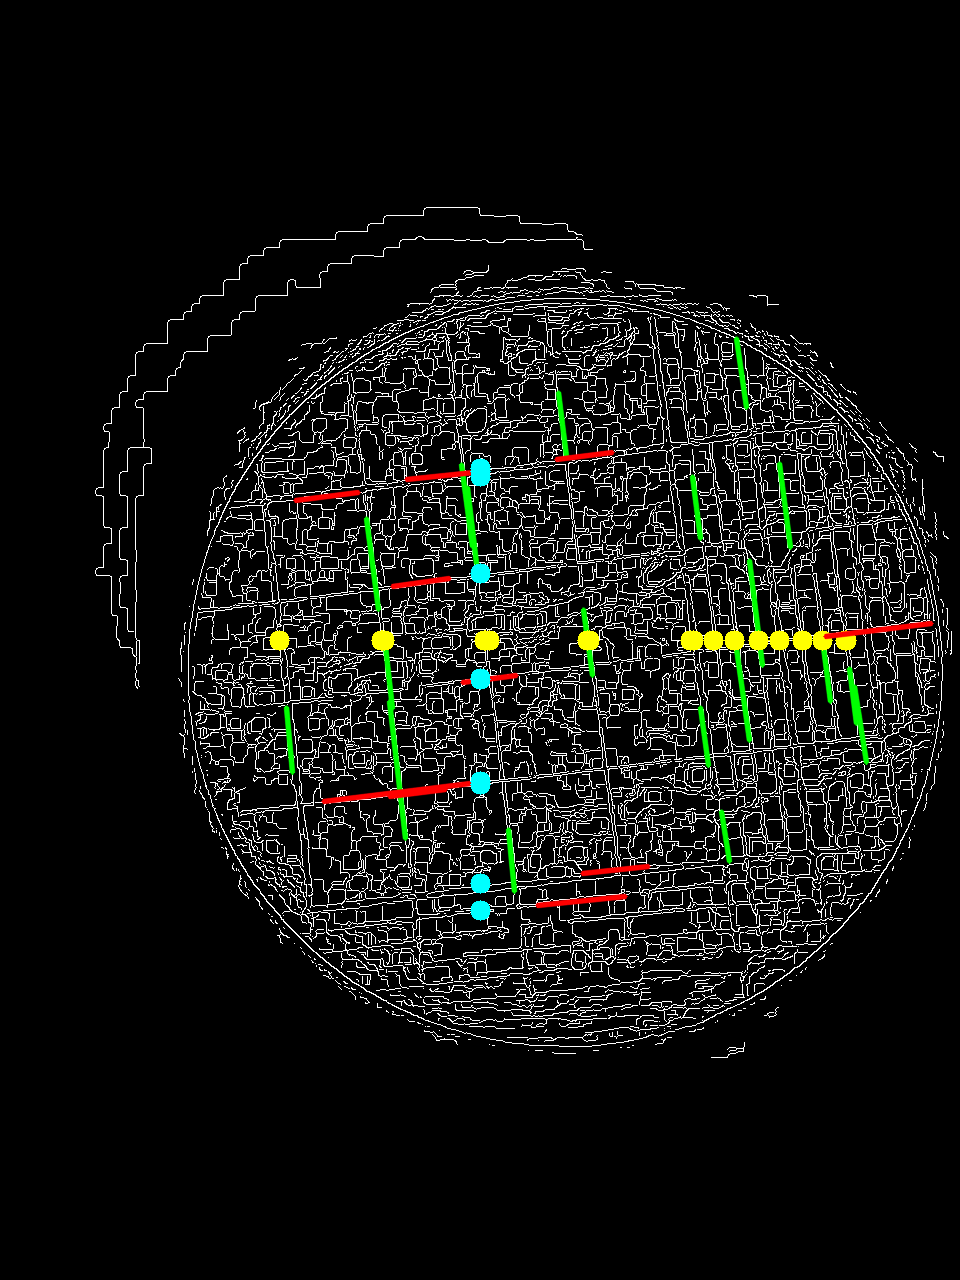
\includegraphics[width=0.31\textwidth]{2022_ConteoMicroAlgas/figs/04_LineasProbabilistico}&
         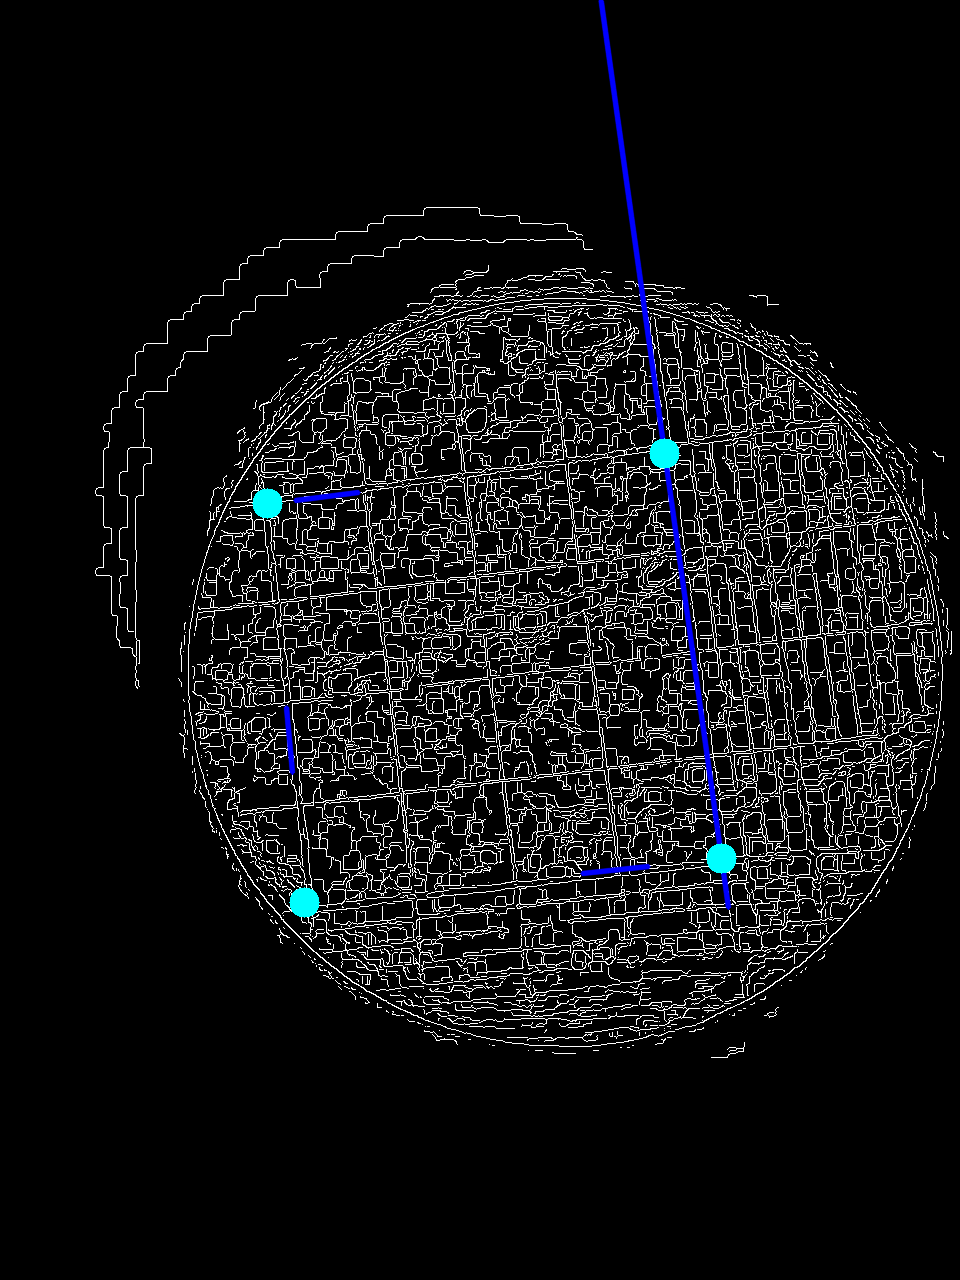
\includegraphics[width=0.31\textwidth]{2022_ConteoMicroAlgas/figs/05_Delimitacion}&
         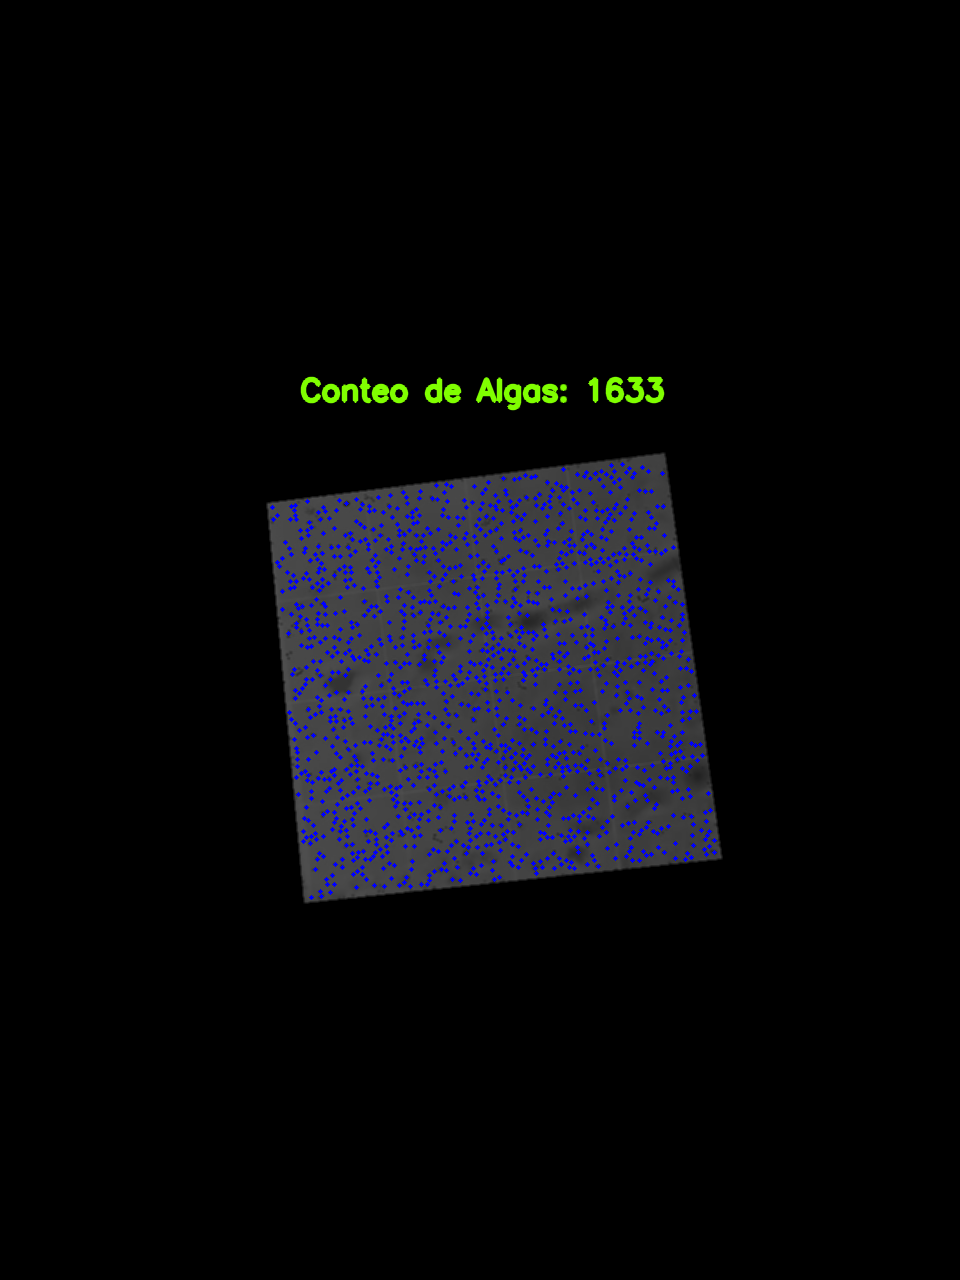
\includegraphics[width=0.31\textwidth]{2022_ConteoMicroAlgas/figs/07_ResultadoConteo}\\

          \end{tabular}
\end{center}
\end{column} 
\end{columns} 
\end{frame}



\begin{frame}{\citetitle{MarcoNuno_ReporteTecnico2022} (4)}

\begin{itemize}
\item Hay un avance significativo con respecto al prototipo versión PC (cerca de completarse)
\begin{itemize} 
\item Se requieren más imágenes, que incluyan el conteo realizado de manera manual para contrastarlo con nuestros algoritmos
\item Posiblemente se deban afinar los algoritmos que se tienen desarrollados
\end{itemize}
\item Con respecto a la fase en el teléfono inteligente, se lleva un avance del 20\%, a reserva de la incorporación de un estudiante de estancia o estadía
\item Los resultados apuntan que es posible publicar los resultados en una Revista Indexada por el JCR
\end{itemize}
\end{frame}




